\title{Assignment 5 - Modeling of infectious diseases\\Epstein-Barr Virus}
\author{
        Leonhard Hauptfeld\\
        MME2 - Bioinformatics
}
\date{\today}

\documentclass[12pt]{article}
\usepackage[english]{babel}
\usepackage[pdftex]{graphicx}

% Set \parskip to put 10pt between paragraphs
\setlength{\parskip}{10pt}

% Set the value of \parindent to 0pt
\setlength{\parindent}{0pt}

\usepackage[a4paper,
            bindingoffset=0.2in,
            left=1cm,
            right=1cm,
            top=1cm,
            bottom=1cm,
            footskip=.25in]{geometry}

\usepackage{multirow}

\usepackage{newunicodechar} % To write the definition on the next line
\newunicodechar{α}{\ensuremath{\alpha}}
\newunicodechar{β}{\ensuremath{\beta}}
\newunicodechar{γ}{\ensuremath{\gamma}}

\usepackage{titling}
\setlength{\droptitle}{-2cm}

\usepackage{outlines}
% Good underlining with \ul instead of shitty LaTeX \underline
\usepackage{soul}

% References
\usepackage[style=ieee]{biblatex}
\addbibresource{A5_Hauptfeld_Leonhard.bib}

\begin{document}
\maketitle

\section{Basic Information}

The Epstein-Barr virus is a widely spread virus proven to be the root cause of
infectious mononucleosis (mono). Recently, a strong association with Multiple Sclerosis
was also found.\cite{EBVMSSurvey} In an analysis of the UK population, antibodies were found in around 95\% 
of people.\cite{EBVSurvey}

A virus of the herpes family, it is commonly spread through saliva and genital secretions.

\section{Modeling}

As there is a fair amount of evidence and modeling research regarding EBV epidemiology
originating in the UK, spread is modeled in UK population. The modeling
includes two scenarios, an unimpeded spread and one with a vaccine intervention. 

The base case includes an already very high number of recovered infected. In a study in the early 2000s, 85.3\% of individuals between 0-25 in the UK tested
positive for presence of EBV. \cite{ebvprevalence} Applying this to to the total number of people aged 0-25 in the UK (17237768) \cite{census}, the base case is 14703816 already recovered people.
Around 45\% of British women aged 16-19 have responded to have had intimate contact within the last week in a survey conducted from 2011 to 2015. \cite{rate} Assuming one in 100 contacts
is sufficiently infectious, the contact rate will be set at 0.45\%. From contracting EBV, it takes around 6 months to either have had mono or having avoided that fate, so the average recovery rate is set at 180 days.

\clearpage
\subsection{Spread without intervention}

For a baseline spread analysis using the SIR model, the aforementioned parameters were entered into a solver. The resulting graph is as follows:

\begin{figure}[!htbp]
	\centering
	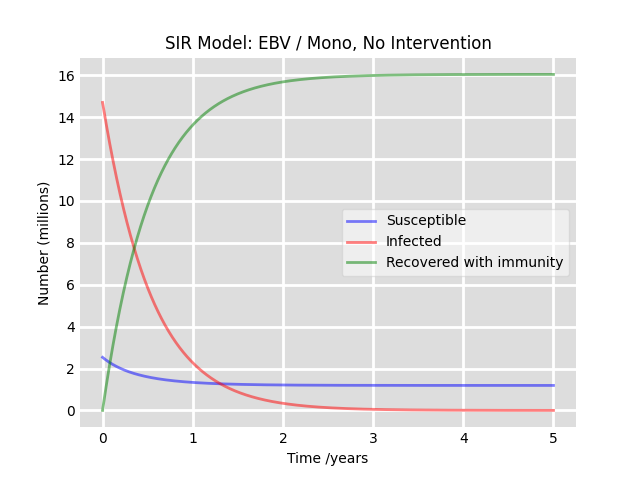
\includegraphics[width=0.5\linewidth]{no_intervention.png}
	\caption{SIR model - No intervention}\label{no_intervention}
\end{figure}

The recovered count jumps up rapidly, as no people have been put in as already recovered, since that
would make them non-infectious according to the SIR model. A small portion of susceptible people
is infected, but once every infected person has recovered a small percentage of non-infected remain. The end-state
is a fairly accurate representation of the EBV "status quo", though probably not due to accuracy of the model.

\subsection{Spread with intervention}

The only vaccine currently available for a herpesvirus like EBV is for the Varicella-zoster virus (ZVZ). The vaccine is 85\% effective at one dose and 98\% effective at two doses,
with a protective period of 8 and 10 years respectively.\cite{ZVZ} The SIR model was adjusted with an amount of vaccinated people (V), creating an SVIR model, based on a found study. \cite{model}
With a vaccine efficacy set at 85\%, the following result was obtained:

\begin{figure}[!htbp]
	\centering
	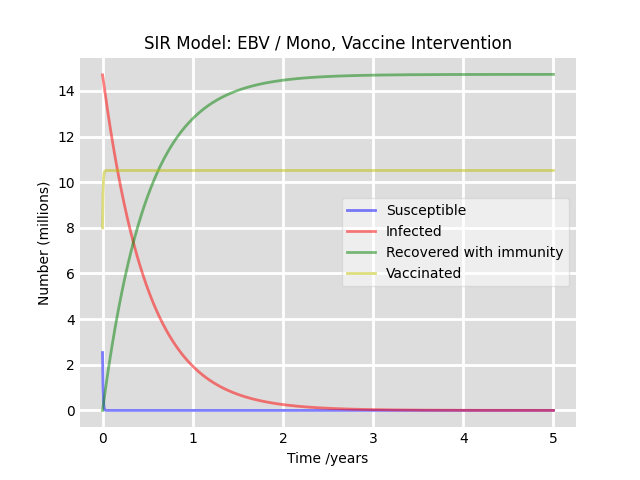
\includegraphics[width=0.5\linewidth]{vaccine_intervention.png}
	\caption{SVIR model - Vaccine intervention}\label{vaccine_intervention}
\end{figure}

An initial vaccinated rate of 8000000 people shows an extremely rapid drop in susceptible people. While obviously
of no help to people already infected, it would be quite a help to the remaining population. This is more or less indicative
of what real research shows in this regard - vaccinating adults proves without desired effectiveness because EBV is already
so prevalent.

\section{Discussion}

This is, by all accounts, a very rough approach to modeling and would require extensive statistical work to be representative data but it is an interesting
use of the SIR model with a very high initial infection and recovered count. It shows a very (unrealistically) high spread of EBV, suggesting that either the model
is flawed or that young adults lie about the amount of intimate contact they have. It also does not account for a large variety of factors, such as actual rate of transmission
when intimate contact occurs as well as new population being born, especially when modelling over such a large period. For a more complete model, different age groups and
their interaction would also have to be taken into account as, in the case of EBV, the incidence rates differ significantly between them.

The introduction of a hypothetical vaccine based on how well the ZVZ vaccine works is an interesting thought experiment, but again, the previously mentioned lack
of sophistication hinders the modelling in this regard.

\subsection{$R_{0}$ vs $R_{e}$}

$R_{0}$ represents the total contagiousness of a disease, including viral (transmission rate, infectious period) human factors. As such this number can vary per area, based
on social customs etc. It is estimated as if everyone in the population was susceptible.

$R_{e}$, the "effective reproduction number", is the total number of people a single individual can infect.
It depends on disease, amount of people a human is in contact with, etc.\cite{RoRe}

\printbibliography

\end{document}
